\documentclass{standalone}
\usepackage{tikz}


\begin{document}

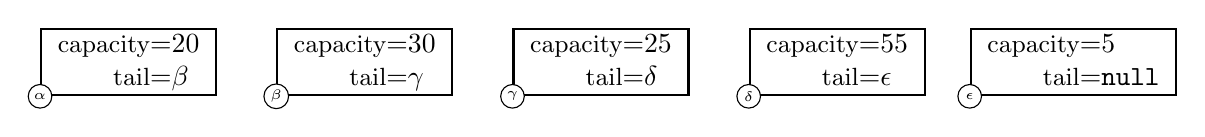
\begin{tikzpicture}[wagon/.style={minimum width=1.2cm,minimum height=0.6cm,draw,black,thick},
                    link/.style={-latex,thin},
                    address/.style={font=\tiny,circle,draw,thin,fill=white,inner sep=1pt,minimum size=3mm}]

  \foreach[count=\i] \c/\address/\tail in {20/\alpha/\beta,30/\beta/\gamma,25/\gamma/\delta,55/\delta/\epsilon,5/\epsilon/{\tt null}} {
    \pgfmathparse{(\i-1)*3}\let\x\pgfmathresult
    \node[wagon,inner sep=0mm] (w\i) at (\x,0) {
      \begin{tabular}{r@{=}l}
        \small capacity & \c \\
        \small tail & $\tail$ \\
      \end{tabular}
    };
    \node[address] at (w\i.south west) {$\address$};
  }
\end{tikzpicture}

\end{document}